As this project is focused on the resource management framework, I will
not give a detailed description of the Hadoop Distributed File
System. Yet, I will go through some basic concepts that will make the
reader understand better the overall architecture of Hadoop.

HDFS is the distributed file system of Hadoop platform. It is designed
with the assumption that hardware failure is the norm and not an
exception making it highly fault-tolerant. Also, it is designed to run
on commodity, heterogeneous, low-cost hardware making the setup and provisioning of
a cluster cheaper than in HPC. HDFS has two main entities, the NameNode
(NN) and the DataNode (DN) and its architecture is depicted in Figure
\ref{fig:hadoop_hdfs}.

\begin{figure}
\centering
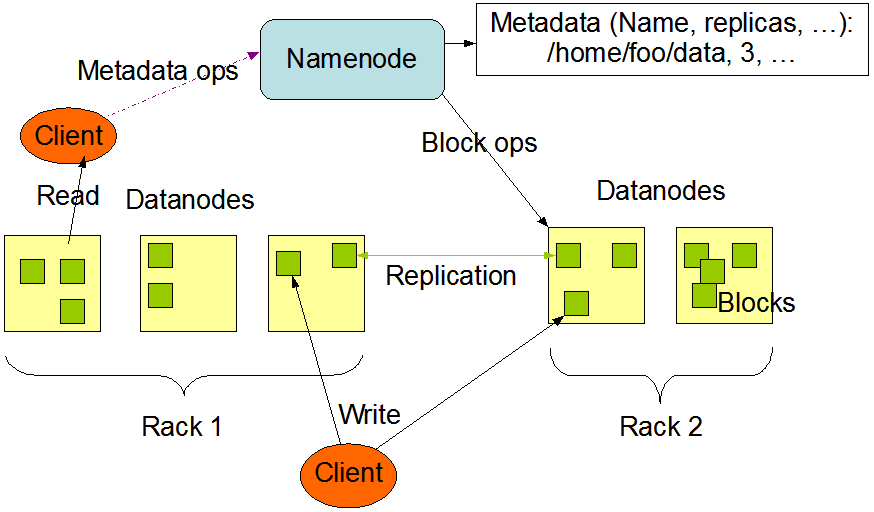
\includegraphics[scale=0.7]{resources/images/Background/hdfs_arch.png}
\label{fig:hadoop_hdfs}
\caption{HDFS architecture}
\end{figure}

\subsubsection{NameNode}
\label{sssec:nn}

An HDFS cluster consists of a single active NN that is responsible for the
file system metadata, the blocks replication and the health
status of the DNs.

HDFS exposes to a user a file system similar to POSIX, in terms that
the structure is hierarchical, there are the same file permissions 
and a subset of POSIX operations. A user through the NN can open,
close, read, delete a file as in any file system. The NN uses a transaction
log, the \emph{EditLog}, that persists to the local file system any
operation that is done to the HDFS namespace. For example if a file is
renamed then a record is added to the EditLog, or if the replication
factor for a file is changed.

As HDFS was designed to run on commodity
hardware it should be able to handle machine failures. Internally, a
file is split in a number of blocks. Typically each block is 128 MB,
except from the last one and are stored
in the DNs. HDFS replicates the blocks to other machines--DNs
according to a configurable replication factor and replication policy.
If the DN that holds a specific block has crashed, then that block is read from
another replica in another DN.
The NN keeps a file in its local file system with the entire namespace
and the mapping of blocks to DNs, called \emph{FsImage}. Upon
recovery, the NN reads the FsImage and applies any operation that is
logged in the EditLog. That way it can recover from a scheduled
maintenance reboot or from a crash.

The NN periodically receives heartbeats from the DNs that have dual
purpose. The first one is to maintain a health status for the DNs. If
the NN misses a heartbeat from a DN, then it marks that DN as
dead. From that point no blocks will be further assigned to that DN
and NN will start migrating all the blocks that reside in that DN to
others. The second reason of receiving heartbeats is to maintain an
updated view of the \emph{BlockMap}, the mapping of blocks to
DNs. When a DN sends a heartbeat to the NN, it piggybacks a list with
the blocks that it currently stores. That way, the BlockMap in the NN
is kept up-to-date with the blocks that are stored in every DN.

\subsubsection{DataNode}
\label{sssec:dn}

Here I will briefly describe the DataNode
